\subsubsection{Pressure Configuration Clamp Design}

The drawings below outline the pressure configuration clamp, two are required. Two of these can be fixed together on a stand to provide a clamp for the pressure sensor syringes. 
The four bolt and nut holes allow the two parts to be clamped together around the upright support. The internal nut holes and through bolt holes allow a single bolt ant nut to act as grub screws to fix the two syringes in place and fix the clamp to the upright support. The single nut and bolt hole  at the end of the part clamps the two parts together so that the syringe grub screws do not splay the parts. 


\begin{figure}[h]
    \centering
    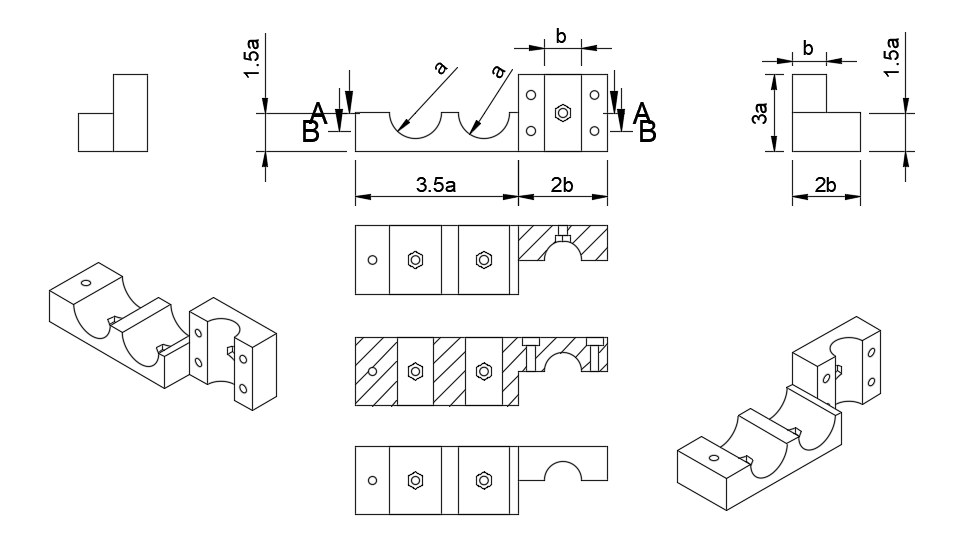
\includegraphics[width=0.7\textwidth]{Figures/SupportDrawings/pressure_conf_clamp_drawing.png}
    \caption{Pressure Syringe Clamp Drawings}
    \label{fig:pressuresyringeclampdrawing}
  \end{figure}


\begin{enumerate}
  \item[a)] The diameter of the pressure syringe + \textgreater\ 4mm
  \item[b)] The diameter of the upright stand/trolley + \textgreater\ 4mm
  \item[Nb)] Select bolts that are greater than the larger of 3a and 3b
  \item[Nb)] Create holes to accommodate the chosen bolts
  \item[Nb)] Create hexagonal holes to accommodate the corresponding nuts, a tight fit makes it easier to move the bolts without the nuts dropping out
\end{enumerate}
